\documentclass[12pt, oneside]{article}
\usepackage{graphicx} %loads the graphicx.sty package 
\usepackage{url}
\usepackage{natbib} 
\usepackage{framed} 

\oddsidemargin 0.1in \topmargin -0.5in \textwidth 6.3in \textheight
9.in

\begin{document}
\title{Predicting the Present with Google Trends}
\author{Hyunyoung Choi\footnote{email: hyunyoung@google.com},   $~$  Hal Varian} 
\date{\today}

\maketitle

\begin{abstract}\noindent We describe how to use search engine query
  data for nowcasting economic time series.  Examples include
  automobile sales, housing sales, unemployment claims, and travel
  destination planning.
\end{abstract}

\newpage

\begin{itemize}
\item Start at t=6, not t=2
\item Update all regression results
\end{itemize}

\noindent In this paper we show how search engine queries be used to estimate
the current level of economic activity.

There are many public and private data releases that report various
measures of current economic activity.  However, these data
are only available with a reporting lag of 1-2 weeks and are often
revised several months later.  For many purposes it would be
attractive to have more timely estimates of these economic indicators.

% \footnote{See, for example, the
% Federal Reserve Economic Data (FRED) available at
% \url{htt://research.stlouisfed.org/fred2/}.}

Google Trends is a service that provides a real-time daily and weekly
index of the volume of queries that users enter into Google.  We have
found that this query data may be correlated with the current
level of economic activity of various sorts and thus may be helpful
for short-term economic measurement.

We are not claiming that Google Trends data can help predict the {\it
  future.\/} Rather we are claiming that Google Trends may help in
{\it predicting the present.}  For example, the volume of queries on
automobile sales during the second week in June may be helpful in
predicting the monthly June sales report for that brand, when it is
released several weeks later in July.

It may also be true that June queries help to predict July sales, but
we leave that question for future research, as this depends very much
on the particular time series in question.  We have found that queries
can be useful leading indicators for subsequent consumer purchases in
situations where consumers start planning purchases significantly in
advance of their actual purchase decision.

Predicting the present, in the sense we described above, is a form of
``contemporaneous forecasting'' or ``nowcasting,'' a topic which is of
particular interest to central banks and other government officials.
As \cite{Castle09} points out, contemporaneous forecasting is valuable
in itself, but also raises a number of interesting methodological and
research questions involving topics such as variable selection, mixed
frequency estimation, and incorporation of data revisions, to name
just a few.

We believe that search engine data such as that available through
Google Trends can be helpful for nowcasting economic data.  Our goals
in this presentation are to familiarize readers with Google Trends
data, illustrate some simple forecasting methods that use this data,
and encourage readers to undertake their own analyses.  

We do not claim any methodological advances here; certainly it is
possible to build more sophisticated forecasting models than those we
use.  However, we believe that the models we describe can serve as
baselines to help analysts get started with their own modeling efforts
and that can subsequently be refined for specific
applications.\footnote{This paper is a much simplified and streamlined
  version of our earlier working papers, \cite{Choi09a,Choi09b} which
  includes other more sophisticated models.}

Our examples use {\tt R}, a freely available open-source statistics
package from \url{http://CRAN.R-project.org}.  We provide the {\tt R}
source code and data in the online appendix available at \url{http:to
  be provided}.

\section{Literature review}

So far as we know, the first published paper that suggested that web
search data was useful in forecasting economic statistics was
\citet{Ettredge05}, which examined the U.S. unemployment rate.  At
about the same time \citet{Cooper05} described using internet search
volume for cancer-related topics.

\citet{Polgreen08} and \citet{Ginsberg09} showed that search data
could help predict the incidence of influenza-like diseases.  This
work was widely publicized and stimulated several further findings in
epidemiology, including \citet{Brownstein09}, \citet{Corley09},
\citet{Hulth09}, \citet{Turbelin09}, \citet{Valdivia10},
\citet{Wilson09}.

\citet{Choi09a, Choi09b} described how to use Google Search Insights
data to predict several economic metrics including initial claims for
unemployment, automobile demand, and vacation destinations; this
report is an updated and streamlined version of those working papers.
\citet{Askitas10}, \citet{Damuri10}, \citet{Suhoy09} examined
prediction unemployment in the US, Germany and Israel.
\citet{Guzman11} has examined Google data as a predictor of inflation.

Recently, \citet{Baker11} have used Google search data to examine how job search responded to extensions of unemployment payments.

\citet{Radinsky09}, \citet{Huang10}, and \citet{Preis10} examine the
use of search data for measuring consumer sentiment while
\citet{Schmidt09} and \citet{Lindberg11} examine retail sales and
consumption metrics.  \citet{Wu10} examine housing data using
longitudinal data extracted from Google Search Insights.

\citet{Shimshoni10} describe the predictability of Google Trends data
itself, pointing out that a substantial amount of search terms are
highly predictable using a simple seasonal decomposition.

\citet{Goel10} provide a useful survey of work in this area and
describe some of the limitations of web search data.  As they point
out, search data is easy to acquire and is often helpful in making
forecasts, but generally may not provide dramatic increases in
predictability.  Although we generally agree with this view, we
typically find economically significant, if not dramatic, improvements
using search engine data, as illustrated in this paper.

Finally, \citet{BOE11} summarizes how web search data can be used for
``nowcasting'' by central banks.

\section{Google Trends\label{trends}}  
\pagenumbering{arabic}

Google Trends provides a time series of the volume of queries users
enter into Google in a given geographic area.

Google Trends data does not report the raw level of queries for a
given search term.  Rather, it reports a {\it query index.}  The query
index starts with the {\it query share}: the total query volume for
search term in a given geographic region divided by the total number
of queries in that region at a point in time.  The query share numbers
are then normalized so that they start at 0 in January 1,
2004. Numbers at later dates indicated the percentage deviation from
the (unnormalized) query share on January 1, 2004.

Note that Google Trends data is computed using a sampling method and
the results with therefore a bit from day to day.  Furthermore, due to
privacy considerations, only queries with a meaningful volume from
distinct IP addresses are tracked.  There is a substantial amount of
online help available via links on the site.

This query index data is available at country, state, and metro level
for the United States and several other countries. There are two user
interfaces for Google Trends data, but the most useful for our
purposes is Google Insights for Search (I4S) which is available at
\url{http://www.google.com/insights/search} since I4S allows a
logged-in user to download the query index data as a CSV file.

Figure \ref{Fig:free-shipping} depicts an example from I4S for the
query [free shipping] in Australia. The search share for this query
has shown a significant increase since 2008 and tends to peak during
the holiday shopping season.


\begin{figure}[ht]
\begin{center}
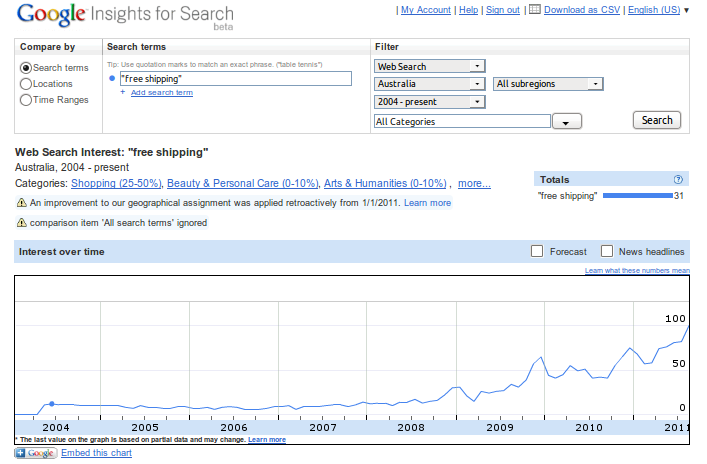
\includegraphics[width= 6.2in]{free-shipping}
\caption{\label{Fig:free-shipping} Search index for [free shipping]} 
\end{center}
\end{figure}

Google classifies search queries into 27 categories at the top level
and 241 categories at the second level using an automated
classification engine.  Queries are assigned to particular categories
using natural language processing methods. For example, the query [car
tire] would be assigned to category {\tt Vehicle Tires} which is a
subcategory of {\tt Auto Parts} which is a subcategory of {\tt
  Automotive.}  These categories are often well aligned with various
economic metrics of interest as demonstrate below.

\section{Examples}

\subsection{Motor vehicles and parts}
As an initial example we use the `Motor Vehicles and Parts Dealers'
series from the U.S. Census Bureau Monthly \& Annual Retail Trade
report.\footnote{\url{http://www.census.gov/retail/marts/www/timeseries.html}.}
This index summarizes results from a survey sent to motor vehicle and
parts dealers that asks about current sales.  The preliminary index is
released 2 weeks after the end of each month.  The data is available
in both seasonally adjusted and unadjusted form; we use the seasonally
adjust data.

Since the series we wish to forecast has been seasonally adjusted, we
need to seasonally adjust the predictors which we do using the
{\tt R} function {\tt stl}.  In general we have found that it is a
good idea use seasonally adjusted predictors for a seasonal index and
unadjusted predictors for a non-seasonally adjusted index.

Let $y_t$ be the log of the observation at time $t$.  We first
estimate a simple baseline AR-1 model $y_t =  b_1y_{t-1} + e_t$.
%\begin{framed}
\small
\begin{verbatim}
            Estimate Std. Error t value Pr(>|t|)    
(Intercept)  0.55343    0.37216   1.487    0.141    
L(y, 1)      0.95023    0.03343  28.423   <2e-16 ***
---
Multiple R-squared: 0.9028,	Adjusted R-squared: 0.9017 
\end{verbatim}
%\end{framed}
\normalsize


Since the coefficient on $y_{t-1}$ is nearly 1 and the intercept term
is not significantly different from zero, the data could easily have
been generated by a random walk.  Indeed, applying an augmented
Dickey-Fuller test indicates that we cannot reject this hypothesis.

It is very common for macroeconomic data to be represented as a random
walk; this was pointed out by \cite{Nelson82} and many subsequent
authors.  For a random walk, the best univariate forecast for $y_t$ is
simply $y_{t-1}$.  However, we can improve on this baseline forecast
by using additional predictors from Google Trends.

Google Trends contains several automotive-related categories.  A
little experimentation shows that several of these categories appear
to add predictive power to this regression.

%\begin{framed}
\small
\begin{verbatim}
                                   Estimate Std. Error t value Pr(>|t|)    
(Intercept)                       2.1307245  0.5924184   3.597 0.000546 ***
L(y, 1)                           0.8117705  0.0525379  15.451  < 2e-16 ***
Auto.Financing                   -0.0014299  0.0005982  -2.390 0.019093 *  
Automotive                       -0.0059722  0.0021867  -2.731 0.007708 ** 
Vehicle.Licensing...Registration  0.0030676  0.0010914   2.811 0.006166 ** 
Vehicle.Shopping                  0.0030547  0.0011456   2.666 0.009213 ** 
---
Multiple R-squared: 0.9173,	Adjusted R-squared: 0.9123 
\end{verbatim}
%\end{framed}
\normalsize

However, the perils of in-sample forecasting are well-known.  The
question of interest is whether the Trends variables improve
{\it out-of-sample forecasting.}

To check this, we look at the one-step ahead out-of-sample forecasts
for $y_t$ using $y_{t-1}$ and the contemporaneous values of the Trends
variables as predictors.  Since the series is actually released 6
weeks after the end of each month, this gives us a meaningful
forecasting lead.

The results are shown in Figure \ref{Fig:autos}.  The mean absolute
forecast error of log($y_t)$ (MAE) using the baseline AR1 model is
0.022, while the MAE using the Trends data is 0.020, an improvement of
about 8.6\%.

\begin{figure}[ht]
\begin{center}
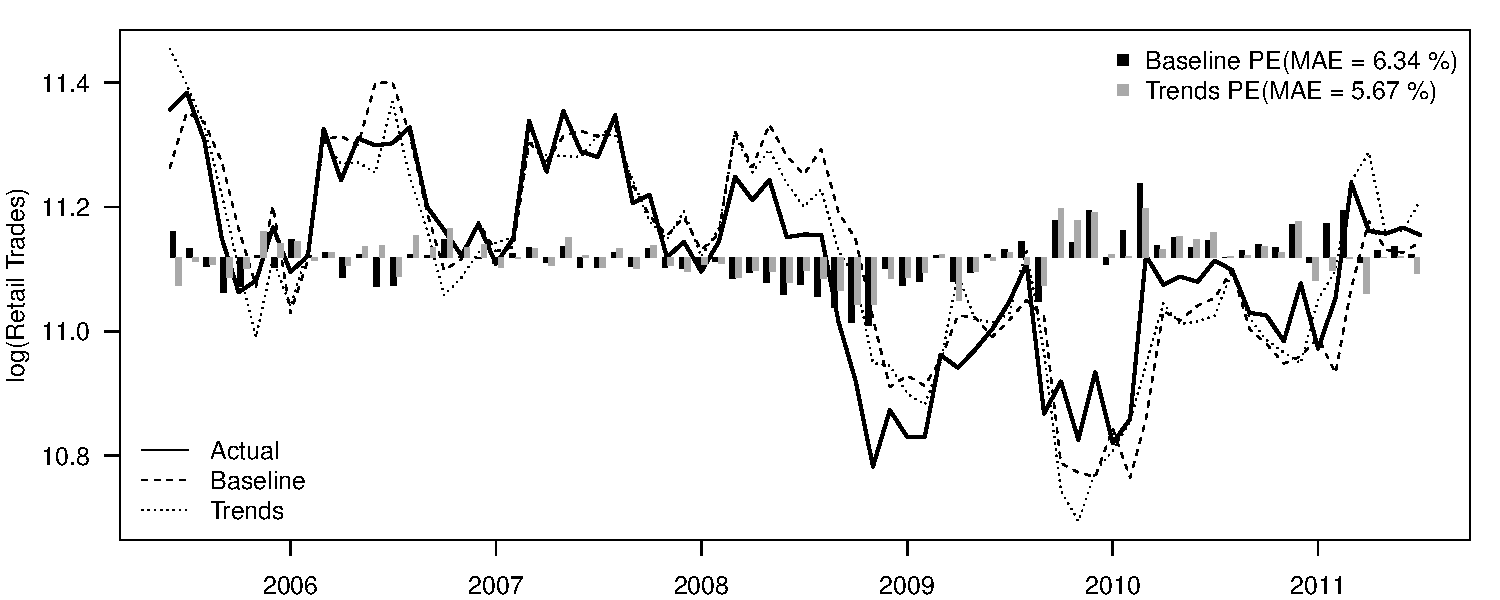
\includegraphics[width= 6.5in]{autos}
\caption{\label{Fig:autos} Motor Vehicles and Parts} 
\end{center}
\end{figure}

Though we have used only predictors from the {\tt Automotive} category
for this example, other categories may also be helpful.  For example,
if we add the `Welfare \& Unemployment' category to the predictors,
the MAE declines to 0.19, a reduction of 13.2\%.   This raises the
thorny question of model/variable selection an issue that can only
become more relevant as data sources such as Google Trends become more
widely available.  See \cite{Castle10} for a recent discussion of
variable selection for nowcasting.

\subsection{New houses sold}

The US Census Bureau and the US Department of Housing and Urban
Development release statistics on the housing market at the end of
each
month.\footnote{\url{http://www.census.gov/const/www/newressalesindex.html}}
The data includes figures on `New Single-Family Houses Sold'; we examine
the seasonally adjusted series and use seasonally adjusted predictors
as described in the previous section.

Again we use a simple autoregression for our baseline forecast of the
log of houses sold.

%\begin{framed}
\small
\begin{verbatim}
            Estimate Std. Error t value Pr(>|t|)    
(Intercept)  0.02524    0.09665   0.261    0.795    
L(y, 1)      0.99382    0.01486  66.891   <2e-16 ***
---
Multiple R-squared: 0.9809,	Adjusted R-squared: 0.9807 
\end{verbatim}
%\end{framed}
\normalsize

As in the previous example, we cannot reject the hypothesis that
$(y_t)$ is a random walk.  But, as before, we find that prediction can
be significantly improved using selection of Google Trends data, in
this case chosen from the Real Estate category.

%\begin{framed}
\small
\begin{verbatim}
                               Estimate Std. Error t value Pr(>|t|)    
(Intercept)                   0.9760482  0.3546423   2.752   0.0073 ** 
L(y, 1)                       0.8509254  0.0526695  16.156   <2e-16 ***
Real.Estate                  -0.0125545  0.0088746  -1.415   0.1610    
Home.Financing                0.0010709  0.0017494   0.612   0.5421    
Home.Inspections...Appraisal  0.0026711  0.0023882   1.118   0.2667    
Home.Insurance                0.0003609  0.0014790   0.244   0.8078    
Real.Estate.Agencies          0.0089980  0.0036766   2.447   0.0166 *  
Rental.Listings...Referrals  -0.0079886  0.0050662  -1.577   0.1187    
---
Multiple R-squared: 0.9832,	Adjusted R-squared: 0.9818 
\end{verbatim}
%\end{framed}
\normalsize

The only statistically significant predictor is {\tt
  Rental.Listings...Referrals}.  However, when we add these variables
to our regressions and compute the one-step ahead out-of-sample
forecast error we find that forecasting performance is significantly
improved by including them.  For the set of predictors shown above we
find that the MAE moves from 0.052 to 0.042, an improvement of 18.5\%.
See Figure \ref{Fig:houses} for the fit.

\begin{figure}[ht]
\begin{center}
\includegraphics[width= 6.5in]{houses}
\caption{\label{Fig:houses} New Houses Sold} 
\end{center}
\end{figure}


\subsection{Initial claims for unemployment benefits}
Each Thursday the US Department of Labor releases a report describing
the number of people who filed for unemployment benefits in the
previous
week.\footnote{\url{http://www.dol.gov/opa/media/press/eta/ui/current.htm}}.

Initial claims have a good record as a leading
indicator. Macroeconomist Robert Gordon indicates that there is a
``surprisingly tight historical relationship in past US recessions
between the cyclical peak in new claims for unemployment insurance
(measured as a four-week moving average) and the subsequent NBER
trough."\footnote{See \url{http://www.voxeu.org/index.php?q=node/3524}
  for details} Furthermore, a cursory inspection of relationship
between Initial Claims and the unemployment rate indicates that
Initial Claims tend to peak 12-18 months before the unemployment rate
peaks.

When someone becomes unemployed it is natural to expect that they will
issue searches such as [file for unemployment], [unemployment office],
[unemployment benefits], [unemployment claim], [jobs], [resume] and so
on. Google Trends classifies search queries like these into two
categories, `Local/Jobs' and `Society/Social Services/Welfare \&
Unemployment'.

As we found in previous cases, the seasonally adjusted weekly initial
claims series tends to follow a random walk.

%\begin{framed}
\small
\begin{verbatim}
            Estimate Std. Error t value Pr(>|t|)    
(Intercept)  0.25488    0.12951   1.968   0.0498 *  
L(y, 1)      0.98022    0.01007  97.368   <2e-16 ***
---
Multiple R-squared: 0.9607,	Adjusted R-squared: 0.9606 
\end{verbatim}
%\end{framed}
\normalsize

Using the Google Trends categories {\tt Jobs} and {\tt
  Welfare...Unemployment} we find a small improvement in the in-sample
fit.

%\begin{framed}
\small
\begin{verbatim}
                        Estimate Std. Error t value Pr(>|t|)    
(Intercept)            1.1843557  0.2743238   4.317 2.01e-05 ***
L(y, 1)                0.9084442  0.0212818  42.686  < 2e-16 ***
Jobs                   0.0007003  0.0003369   2.078  0.03834 *  
Welfare...Unemployment 0.0004828  0.0001831   2.636  0.00872 ** 
---
Multiple R-squared: 0.9623,	Adjusted R-squared: 0.9621 
\end{verbatim}
%\end{framed}
\normalsize

When we look at out-of-sample performance we find that the MAE goes
from 0.033 using the baseline forecast to 0.322 which is only a 2.8\%
improvement.  However, when we look at the series a bit more closely a
rather different picture emerges.

It is well-known that it is difficult to identify ``turning points''
in economic series.  For this particular series there are three
notable turning points, and it is worthwhile examining the reduction
in MAE in the weeks surrounding these dates.  See Figure
\ref{Fig:iclaims}.

\begin{description}
\item[2009-03-01 : 2009-05-01] This is when the series peaked in the
  Spring of 2009 signaling the end of the recession.  MAE using the
  Trends data was 24.3\% lower than the baseline model

\item[2009-12-01 : 2010-02-01] This is when the series stopped
  declining in early 2010. MAE using Trends data went down by 10.3\%
  compared to the baseline.

\item[2011-01-01 : 2011-05-01] This is when the series resumed
  increasing in early 2011.  MAE using trends data went down by 4.8\%
  relative to the baseline.
\end{description}

\begin{figure}[ht]
\begin{center}
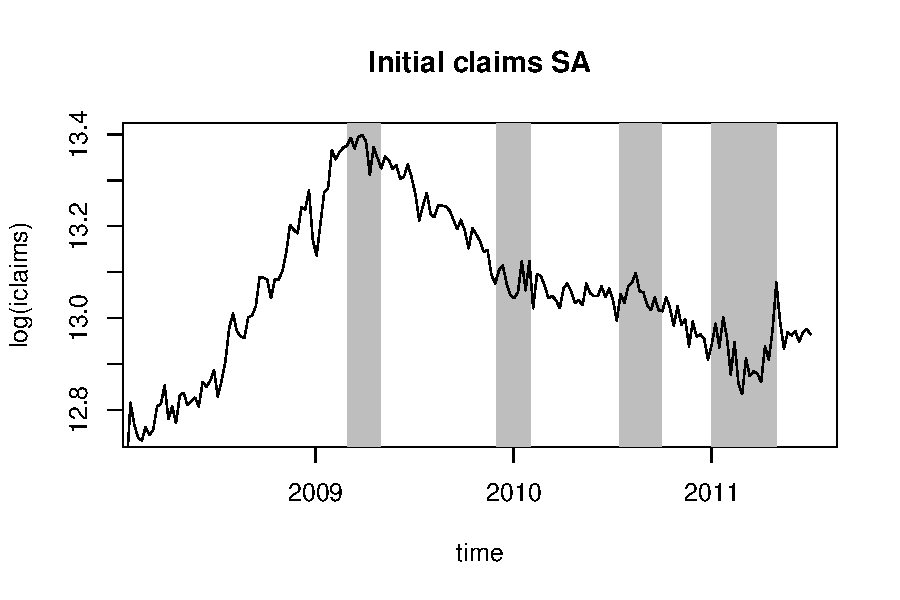
\includegraphics[width=6.5in]{iclaims}
\caption{\label{Fig:iclaims} Initial claims for unemployment; turning
  points in grey.} 
\end{center}
\end{figure}


In this case, the Google Trends data seems to help in identifying
turning points.  \cite{Askitas10}, \cite{Suhoy09}, and \cite{Damuri10}
have confirmed the value of search data in forecasting unemployment in
the U.S., Germany and Israel.

\subsection{Travel} 
The internet is commonly used for travel planning which suggests that
Google Trends data about destinations may be useful in predicting
visits to that destination.  We illustrate this using data from the
Hong Kong Tourism Board.\footnote{\url{http://partnernet.hktourismboard.com}}

The Hong Kong Tourism Board publishes monthly visitor arrival
statistics, including `Monthly visitor arrival summary' by
country/territory of residence. For this study we use visitor data
from US, Canada, Great Britain, Germany, France, Italy, Australia,
Japan and India.

'Hong Kong' is also one of the subcategories in under Vacation
Destinations in Google Trends.  We can examine the query index for
this category by country.

The Hong Kong Visitor Arrival data is not seasonally adjusted, nor is
the Google Trends data.  We used the average query index in the two
observations of the month to predict the total monthly visitors.
Since the data is released with a one-month lag, this gives us roughly
a 6-week lead in terms of forecasting

If we let $y_t$ be the visitors a given country in month $t$, and
$x_t$ be the average Google Trends index for the first two weeks of
that month, we can write a basic model is a seasonal AR-1 model of the
form $y_t = b_1y_{t-1} + b_{12}y_{t-12} + b_0x_{t} + e_t$.

We estimate this model for each country and compare the actual to the
fitted results in Figure \ref{Fig:hk}.  As can be seen, the in-sample
forecasts are pretty good, with the exception of Japan.  Excluding
Japan, the average $R^2$ is over 70\%.  In \cite{Choi09a} we use a
more elaborate random effects model with some additional predictors
and find substantially better in-sample fit.

\begin{figure}[ht]
\begin{center}
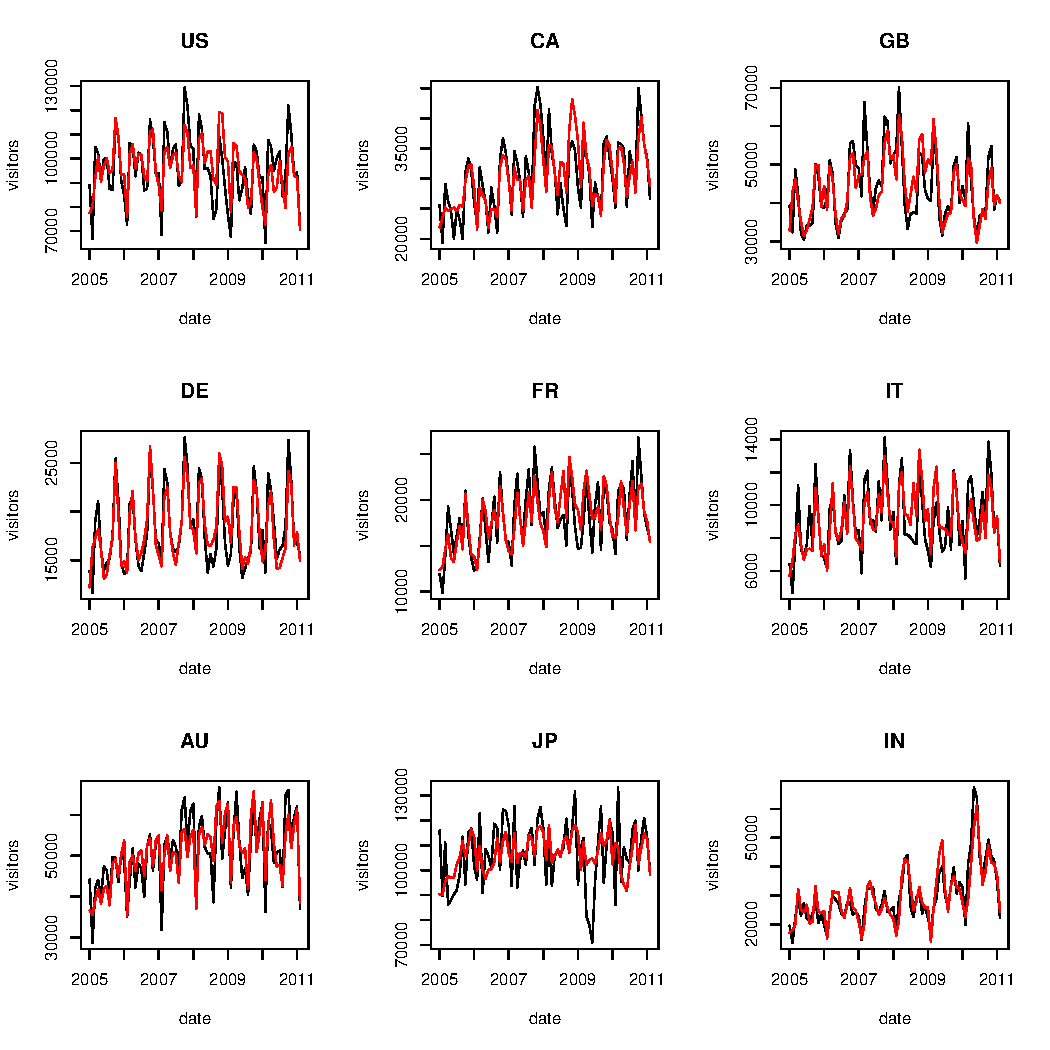
\includegraphics[width= 6.2in]{hk}
\caption{\label{Fig:hk} Visitors to Hong Kong} 
\end{center}
\end{figure}


\section{Conclusion \label{Sec:Conclusion}}  

We have found that simple seasonal AR models that includes relevant
Google Trends variables tend to outperform models that exclude these
predictors by 5\% to 20\%.  We hope that these examples will encourage
other researchers to examine this data source.

Google Trends data is available at a state and metro level for several
countries.  We have also had success with forecasting various business
metrics using state-level data.  It appears that longitudinal data helps
make up for the rather short time series available from Google Trends.

%\section{Bibliography}
\bibliographystyle{plainnat}
\bibliography{i4s}

\end{document}

